%%%%%%%%%%%%%%%%%%%%%%%%%%%%%%%%%%%%%%%%%%%%%%%%%%%%%%%%%%%%%%%%%%%%%%%%%%%%%%%
\section{MGXS Generation}
\label{sec:mgxs-generation}
%%%%%%%%%%%%%%%%%%%%%%%%%%%%%%%%%%%%%%%%%%%%%%%%%%%%%%%%%%%%%%%%%%%%%%%%%%%%%%%

This paper uses Monte Carlo to generate MGXS. A single-step framework used to generate MGXS from Monte Carlo is discussed in~\autoref{subsec:single-step}. Two pin-wise spatial homogenization schemes used to quantify approximation error due to inter-pin spatial self-shielding are introduced in~\autoref{subsec:homogenize}.


%%%%%%%%%%%%%%%%%%%%%%%%%%%%%%%%%%%%%%%%%%%%%%%%%%%%%%%%%%%%%%%%%%%%%%%%%%%%%%%
\subsection{A Single-Step Framework}
\label{subsec:single-step}

In general, MGXS generation schemes use a multi-step approach to decouple the energy, angular and spatial dimensions of the transport equation. The multi-step approach typically applies high-fidelity models of the energy self-shielding physics to low-fidelity geometric models of unique core components as illustrated in~\autoref{fig:multi-step-framework}. The multi-step approach uses a combination of models of varying complexity to optimize overall simulation speed with accuracy. However, this is often done at the expense of generality. For example, multi-step MGXS generation schemes do not typically model inter-assembly physics or the effect of reflectors and other core heterogeneities on the spatial distribution of the flux. Instead, geometric heuristics are often used to embed spatial self-shielding effects in MGXS for similarly shielded spatial zones (\textit{e.g.}, fuel pins with similar neighboring pins). The approximations to the energy and spatial variation of the flux introduce approximation error in full-core calculations and limit the core design parameter space for which multi-step schemes may be applied. 

\begin{figure}[h!]
\centering
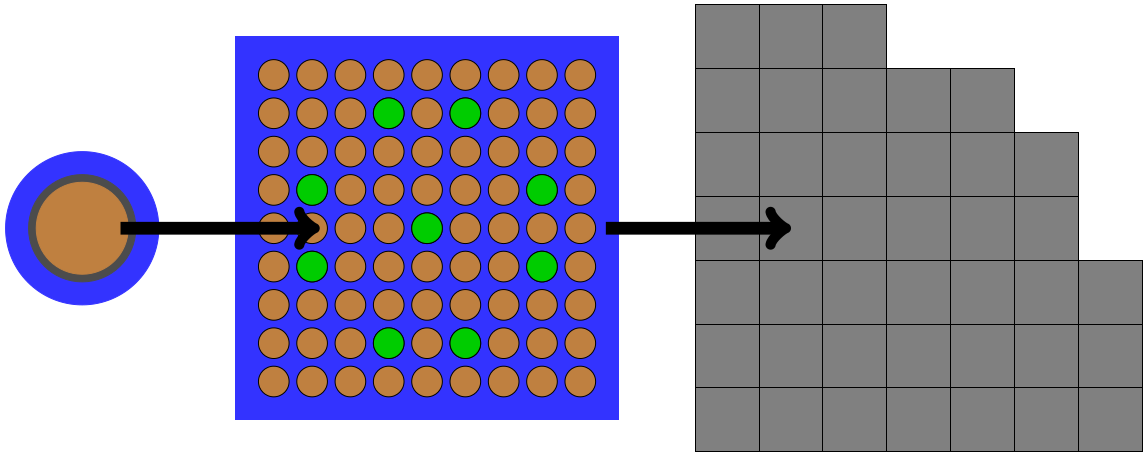
\includegraphics[width=\linewidth]{figures/multi-step-flow-chart}
\caption{The multi-step approach typically used for deterministic reactor physics calculations~\citep{gibson2016thesis}.}
\label{fig:multi-step-framework}
\end{figure}

This paper employs Monte Carlo methods to generate MGXS since they present a natural approach to replace engineering prescriptions to approximate the flux with a stochastic approximation of the exact flux. However, MC-based MGXS generation methods to date have retained the multi-step geometric framework to tabulate MGXS for individual reactor components -- such as infinite fuel pins and/or assemblies -- for subsequent use in full-core multi-group calculations. Although the use of MC within a multi-step framework eliminates the need to approximate the flux in energy, it does not account for spatial self-shielding effects throughout a reactor core. 

This paper abandons the multi-step approach in favor of a single-step framework that uses MC eigenvalue simulations of the complete heterogeneous geometry to simultaneously account for all energy and spatial effects in a single step. The single-step framework may be impractical for MGXS generation for industrial applications since it is constrained by the slow convergence rate of Monte Carlo tallies. Nevertheless, it allows for the rigorous quantification of approximation error due to spatial self-shielding models used to generate MGXS, which is the focal point of this paper.


%%%%%%%%%%%%%%%%%%%%%%%%%%%%%%%%%%%%%%%%%%%%%%%%%%%%%%%%%%%%%%%%%%%%%%%%%%%%%%%
\subsection{Pin-Wise Spatial Self-Shielding Models}
\label{subsec:homogenize}

%-focus less on introducing these as ``schemes'' per se
%  -rather two spatial self-shielding models to quantify approx. error

This paper employs two different spatial homogenization schemes to model spatial self-shielding effects in MGXS. Although all spatial zones may experience spatial self-shielding, this chapter only models the impact of spatial self-shielding on MGXS in fissile regions. The null and degenerate spatial homogenization schemes are introduced in~\autoref{subsubsec:homogenize-null} and~\autoref{subsubsec:homogenize-degenerate}, respectively. These schemes model spatial self-shielding for each fuel pin with increasing granularity. 

%The \texttt{openmc.mgxs} module was used to compute 70-group MGXS with OpenMC for both the assembly and colorset benchmarks. 

%%%%%%%%%%%%%%%%%%%%%%%%%%%%%%%%%%%%%%%%%%%%%%%%%%%%%%%%%%%%%%%%%%%%%%%%%%%%%%%
\subsubsection{Null Spatial Homogenization}
\label{subsubsec:homogenize-null}

The \textit{null} spatial homogenization scheme uses a single Monte Carlo calculation of the complete heterogeneous geometry to generate MGXS for each material. The spatially self-shielded flux is used to collapse the cross sections in each material with a unique isotopic composition. The null scheme does not account for spatial self-shielding effects experienced by different fuel pins filled by the same fuel composition, and instead averages these effects across the entire geometry. A single MGXS is employed in each instance of a material zone, such as a fuel pin replicated many times throughout a benchmark geometry. The null scheme serves as the base case in this paper to illustrate the approximation error which results when inter-pin spatial self-shielding effects are neglected, even when the exact flux from Monte Carlo is used to collapse continuous energy cross sections.

% In this way, the null scheme fully abandons the multi-step approach used by most traditional approaches to generate MGXS.

%%%%%%%%%%%%%%%%%%%%%%%%%%%%%%%%%%%%%%%%%%%%%%%%%%%%%%%%%%%%%%%%%%%%%%%%%%%%%%%
\subsubsection{Degenerate Spatial Homogenization}
\label{subsubsec:homogenize-degenerate}

The \textit{degenerate} spatial homogenization scheme accounts for spatial self-shielding effects experienced by each instance of each fuel pin throughout a heterogeneous geometry. Like the null scheme, a single MC calculation of the complete heterogeneous geometry is used to generate MGXS for all materials. Unlike the null scheme, the MGXS are tallied separately for each instance of fissile material zones. For example, if a heterogeneous benchmark includes $N$ fuel pins, then $N$ collections of MGXS are separately tabulated for each fuel pin instance. The degenerate scheme tallies different MGXS even if the isotopic compositions in the fuel pin instances are identical, since each instance may experience different spatial self-shielding effects and hence have different MGXS. The degenerate scheme demonstrates the reduction in approximation error between multi-group and continuous energy transport methods that can be achieved when inter-pin spatial self-shielding effects are sufficiently modeled in MGXS.
